\documentclass{examen}
\usepackage{listings}
\begin{document}

\modulo{Aplicaciones web -- PARTE ORDENADOR -- SOLO PARTE 2}
\pregunta{Utilizando la herramienta ofim�tica de Google elabora un formulario como el siguiente. Documenta el proceso paso a paso con las capturas de pantalla y las explicaciones del proceso}{2}

\begin{figure}[h]
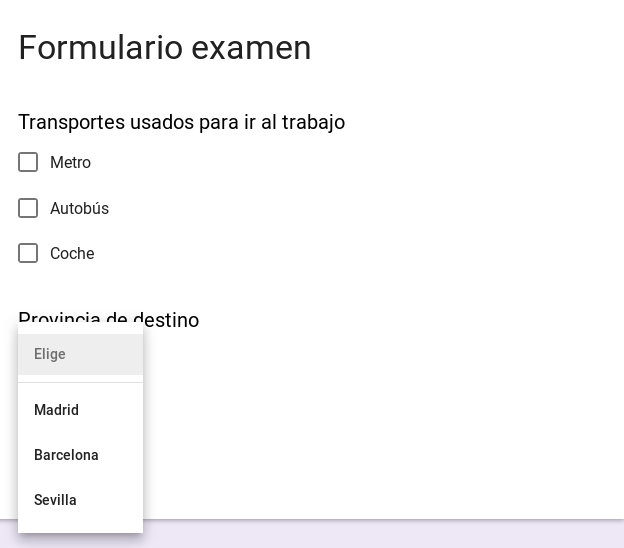
\includegraphics[scale=0.5]{examen-img/formulario.png}
\end{figure}

\break 
\pregunta{Utilizando la herramienta de dibujo de Google elabora un gr�fico exactamente como el mostrado en la figura siguiente. Documenta el proceso paso a paso con las capturas de pantalla y las explicaciones del proceso}{3}

\begin{figure}[h]
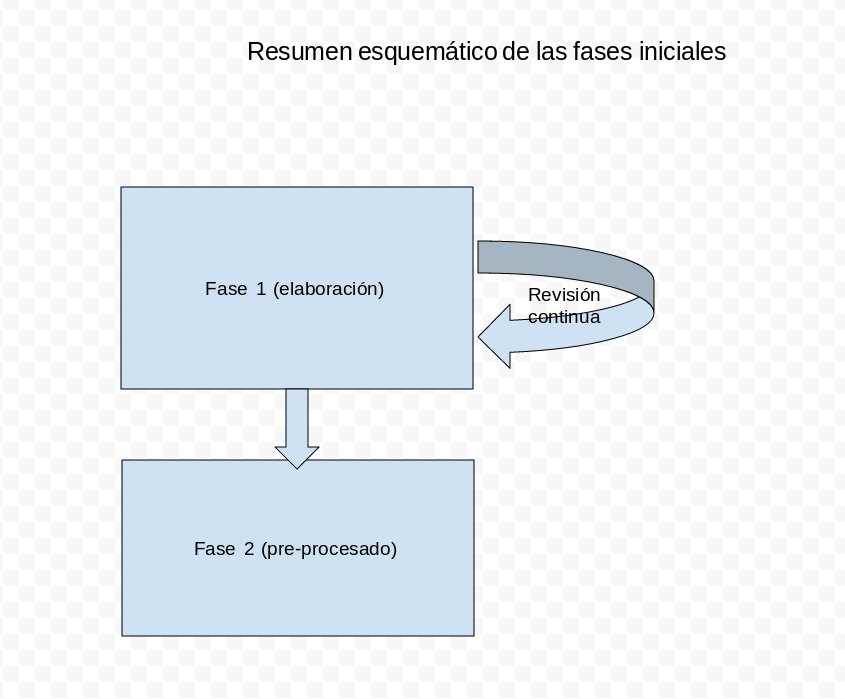
\includegraphics[scale=0.5]{examen-img/dibujo.png}
\end{figure}


\end{document}
